\chapter{Analysis}

In this chapter, I will shortly describe the dataset provided for this task, go over related work and then describe the frameworks and tools that are available. In the end, I draw a conclusion and decide on how to proceed.

\section{Dataset}

The provided dataset consists of about 2'000 microscopic images with and without asbestos fibers. The images come in two different dimensions and different qualities. Most of the images are 1024 by 1024 pixels and using up 1.1 MB of disk space but some are in 1024 by 768 pixels and use only around 700 kB of disk space. The smaller images were originally in TIF format which needed to be converted into PNG format for better being able to load them into python objects. All images are in grey color space. Since all architectures have been originally trained on color images, the image is transformed into an RGB tensor during dataset preparation. All gray space values ranging from 0 to 255 are copied into each channel of RGB. In Figure \ref{fig:asbestos_examples} three images labeled as containing asbestos are shown whereas in Figure \ref{fig:non-asbestos_examples} three images without asbestos are shown.\\


\begin{figure}[h]
\centering
\caption{Three examples of images with asbestos fibers. On the left, the asbestos fibers are clearly visible, in the middle it's much harder to find them. In the right image there might be none, although the image is labeled as having asbestos in it.}
\subfigure{
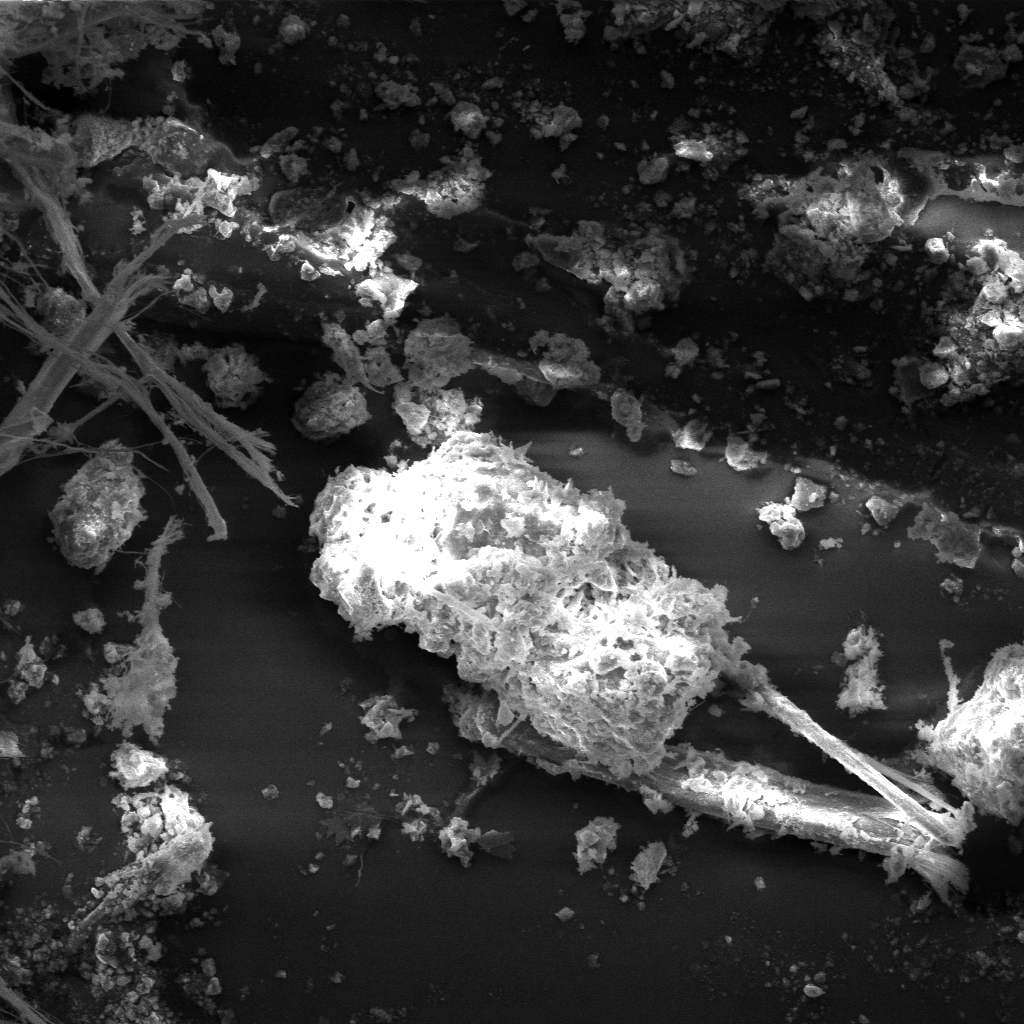
\includegraphics[width=.3\textwidth]{images/chapter2/asbestos_one.png}
}
\subfigure{
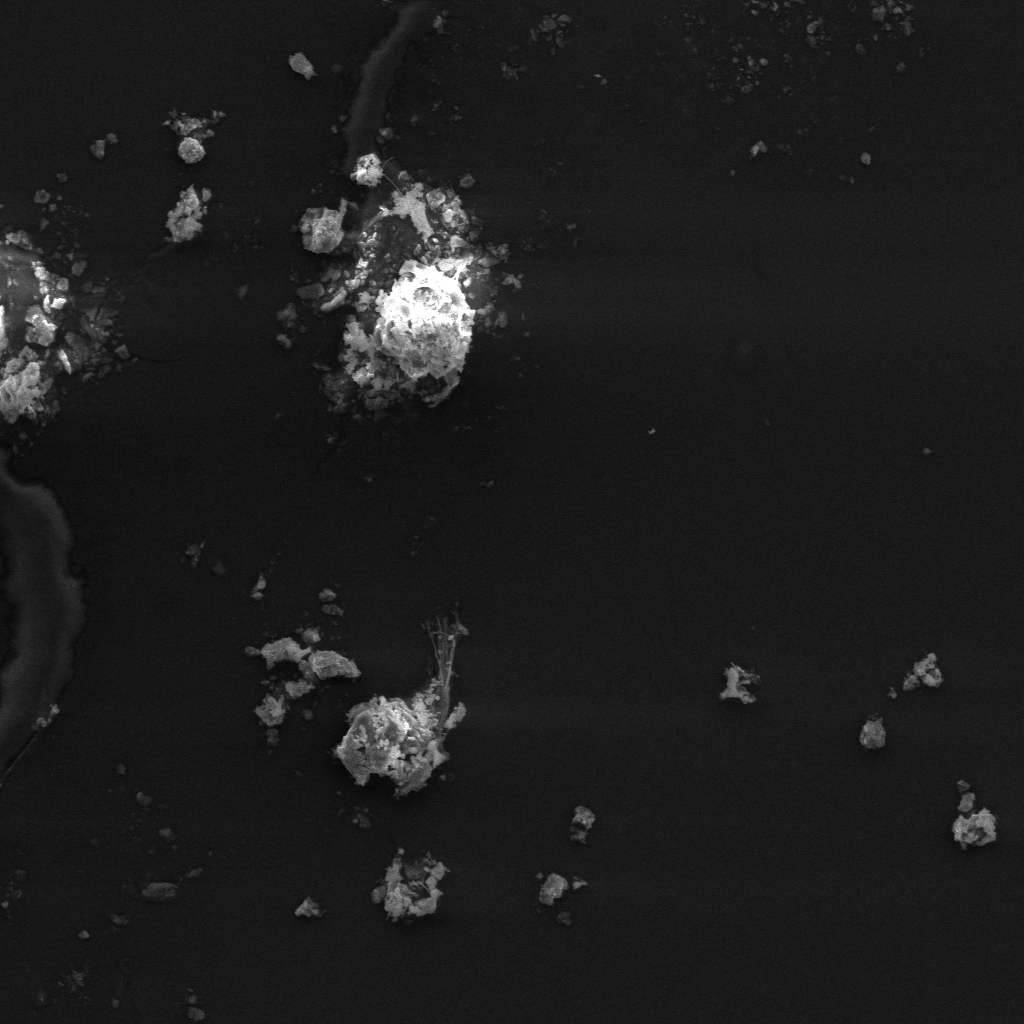
\includegraphics[width=.3\textwidth]{images/chapter2/asbestos_two.png}
}
\subfigure{
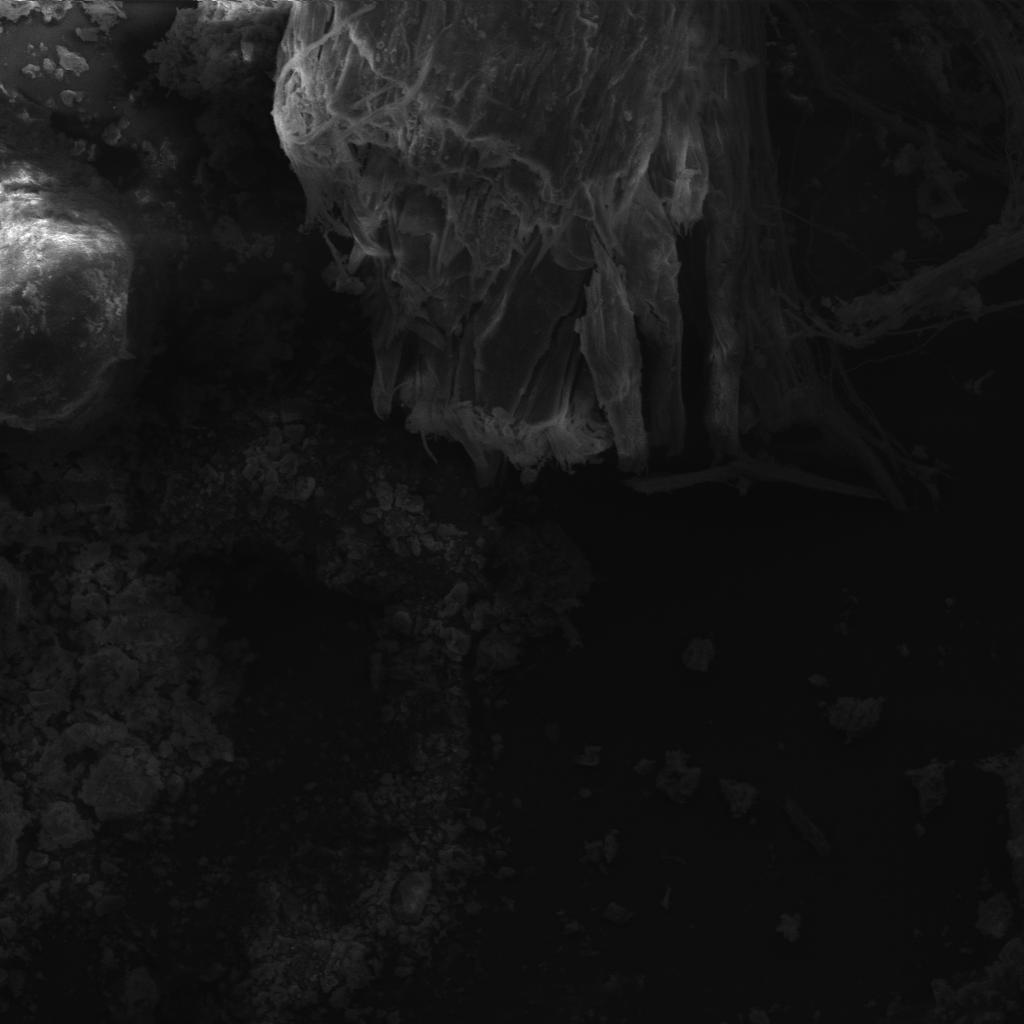
\includegraphics[width=.3\textwidth]{images/chapter2/asbestos_three.png}
} 
\label{fig:asbestos_examples}
\end{figure}

\begin{figure}[h]
\centering
\caption{Three examples of images without asbestos fibers. On the left image, there is clearly no asbestos to be found. In the middle and left image it's already much more difficult to be certain that there are no chrysotile fibers present.}
\subfigure{
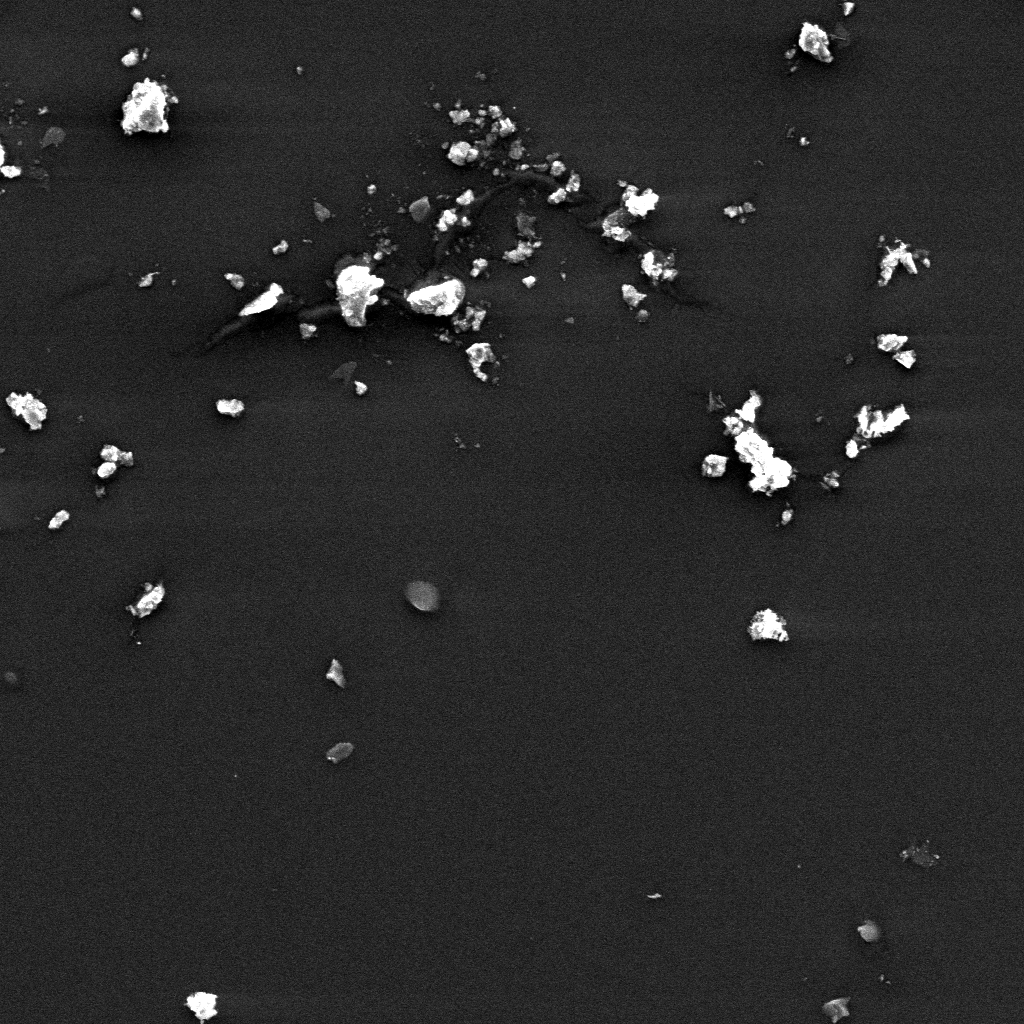
\includegraphics[width=.3\textwidth]{images/chapter2/non-asbestos_one.png}
}
\subfigure{
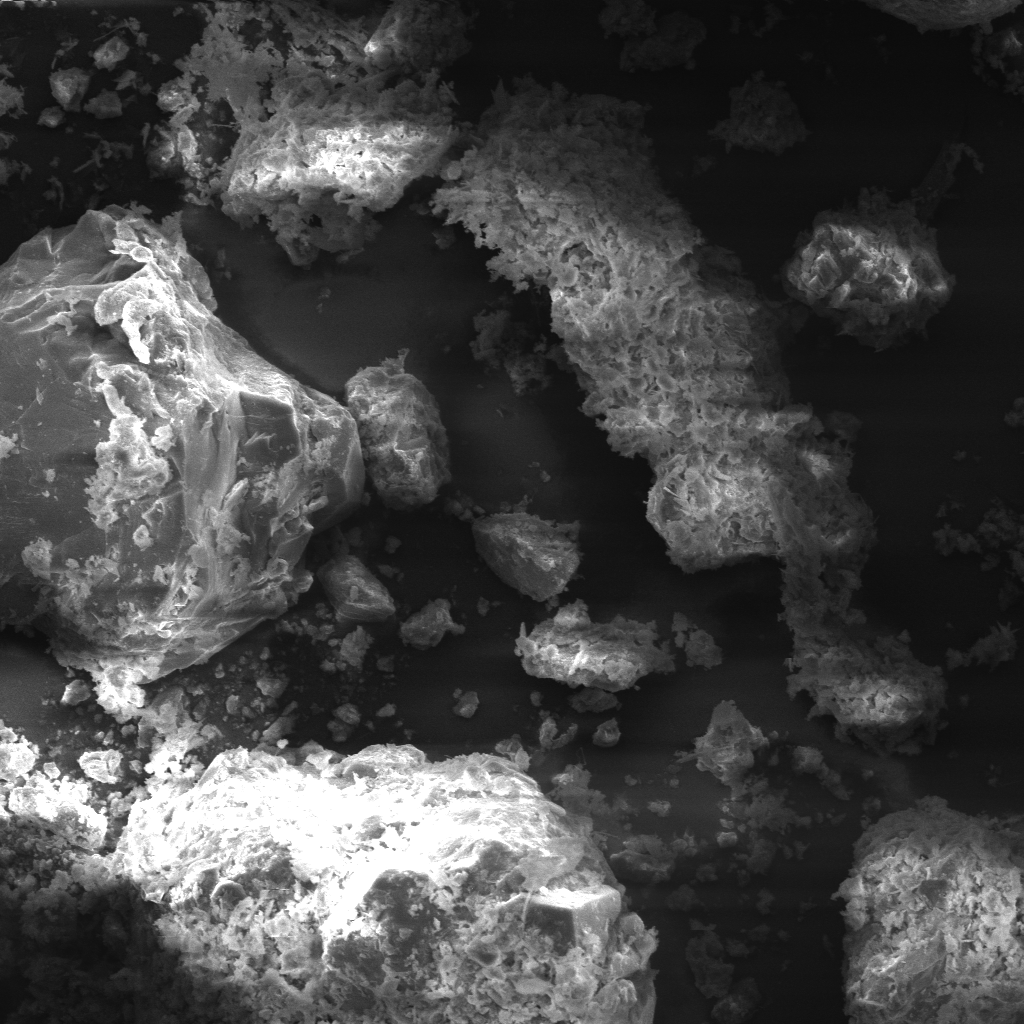
\includegraphics[width=.3\textwidth]{images/chapter2/non-asbestos_two.png}
}
\subfigure{
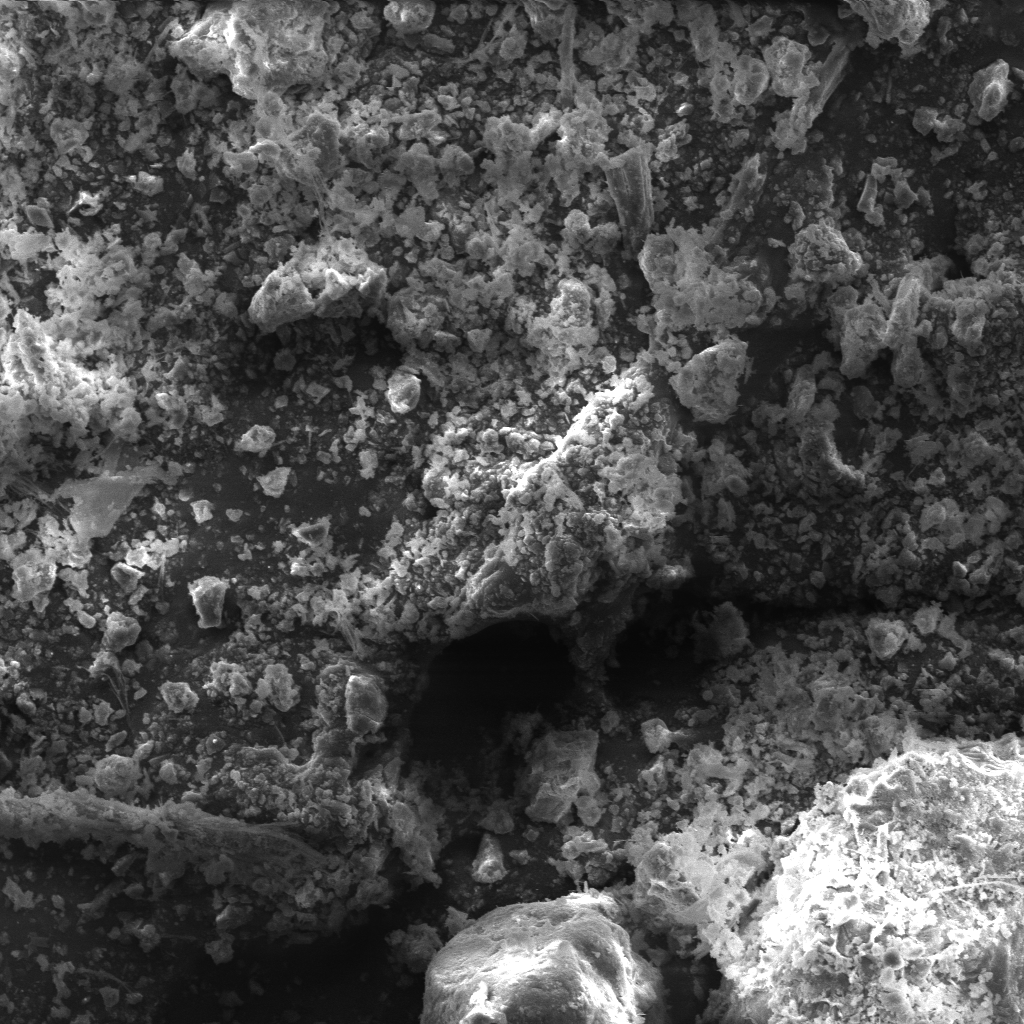
\includegraphics[width=.3\textwidth]{images/chapter2/non-asbestos_three.png}
}
\label{fig:non-asbestos_examples}
\end{figure}

With the dataset a ground truth folder was provided with 116 images pre-labeled as having asbestos fibers in them or not. From these 116 images the remaining images needed to be manually labeled. Some of the later labeled images were checked by the laboratory but Figure \ref{fig:wrong_asbestos_labeling} shows that even that leaves much space for errors.  According to the laboratory, the image shown in Figure \ref{fig:wrong_asbestos_labeling} has no asbestos in it. Nonetheless, there are several areas where asbestos-like structures emerge once the image is made brighter with a photo-editing tool, especially a long fiber on the left side of the image becomes visible and is marked by two arrows. Brightening, sharpening and other simple editing tools are often used prior to classification to make the structures more visible. This is to show, that the labeled data for training will most certainly have errors in it and that some images might look like having asbestos fibers in it but actually don't and the other way around. In the laboratory samples are examined with additional methods to be sure if asbestos is present or not, but that is not part of the master thesis. Therefore one of the main goals of this thesis is to be able to label all images and reduce the manual workload. Uncertain images should be labeled as containing asbestos and if needed examined further by the laboratory. That means that the rate of false negatives should be as low as possible.

\begin{figure}[h]
\centering
\subfigure{
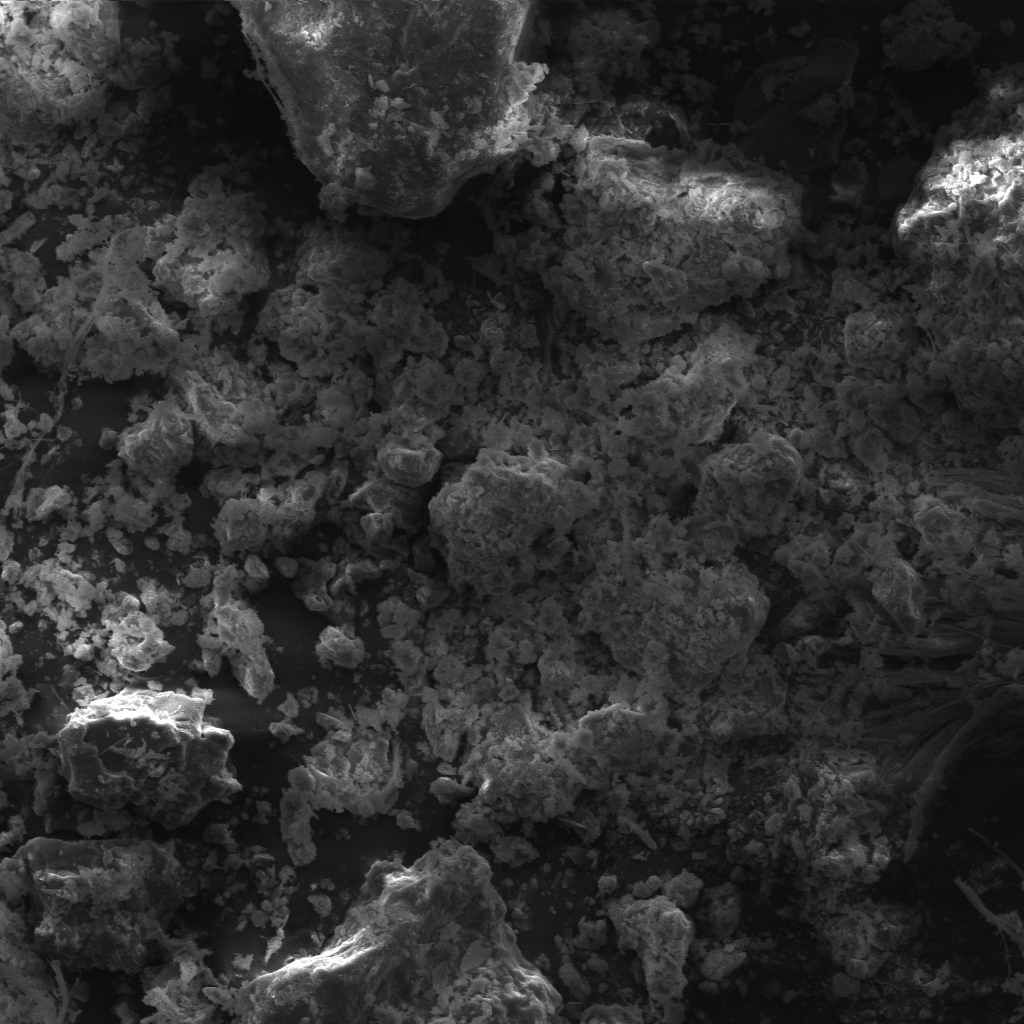
\includegraphics[width=.4\textwidth]{images/chapter2/probably_wrong_label.png}
}
\subfigure{
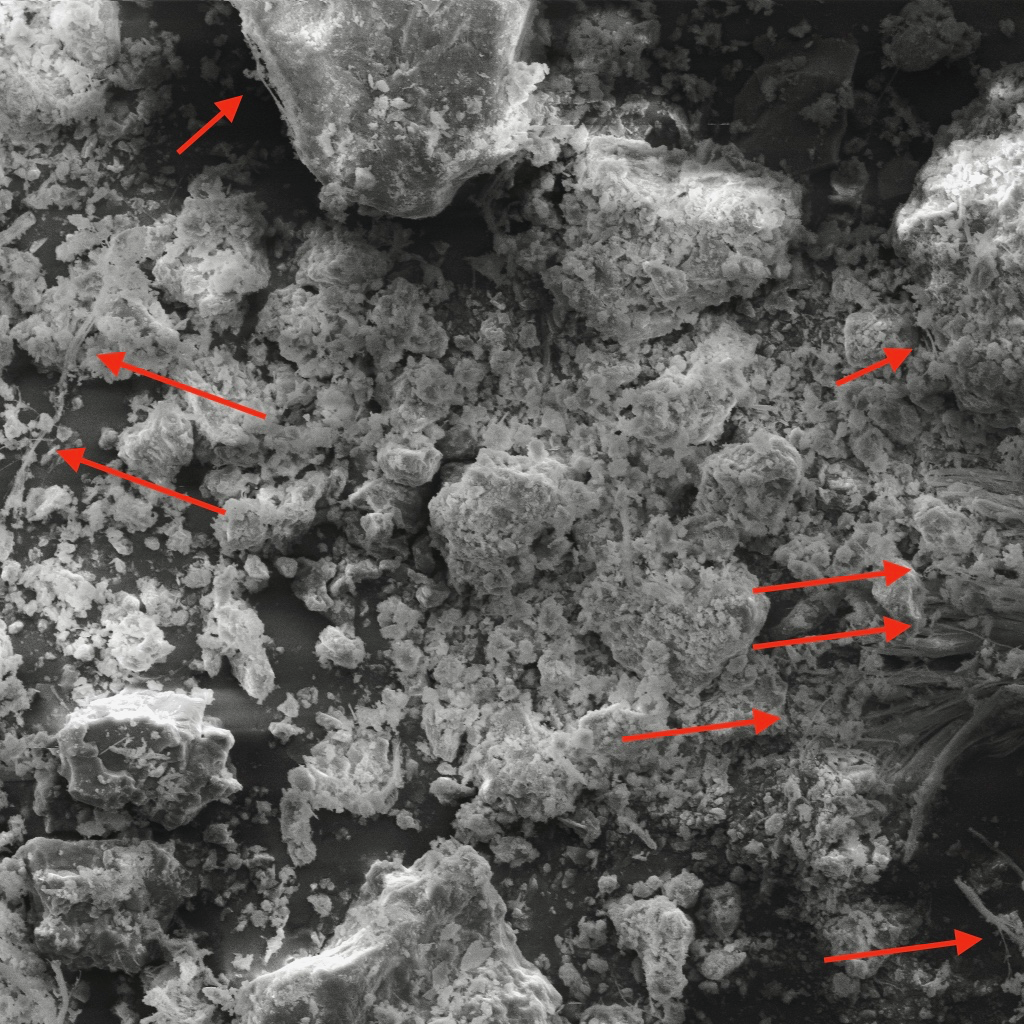
\includegraphics[width=.4\textwidth]{images/chapter2/probably_wrong_label_edited.png}
}
\caption{After brightening up the image and looking at it carefully, many different asbestos like structures emerge.}
\label{fig:wrong_asbestos_labeling}
\end{figure}

\section{Related Work}

There are many different forms of asbestos that occur in different materials and environments, therefore the detection and quantification methods are quite different as well, although most of them are based on microscopic images. After the samples have been collected, trained experts need to quantify and classify the fibers in order to assess the contamination and risk factors to humans since not all asbestos fibers (eg. length, aspect ratio and density) are equally toxic to humans. The structure needs to be manually checked and matched exactly to a set of predefined and standardized characteristics, also called templates. This process is very time intensive and costly and therefore automated detection and counting methods are being developed. The most important and widely used methods for detecting asbestos from air samples are e.g. phase contrast microscopy (PCM), transmission electron microscopy (TEM), scanning electron microscopy (SEM) as seen in Figure \ref{fig:chrysotile}, and polarized light microscopy (PLM) \cite{perry2004discussion}. These techniques are mostly adapted for soil samples although soil samples pose many new problems like standardized preparation of the samples. Air samples are much cleaner and the asbestos fibers can be counted more easily without noise interfering, thus the results are more accurate and counts are rather reproducible. With soil samples, there is much more debris in the samples and getting a homogenous sample out of a bigger object that can generalize to the whole is one of the biggest problems. Figure \ref{fig:sampleprep} shows how a very simple sample preparation could look like. \\

\begin{figure}[h]
\centering

\subfigure{
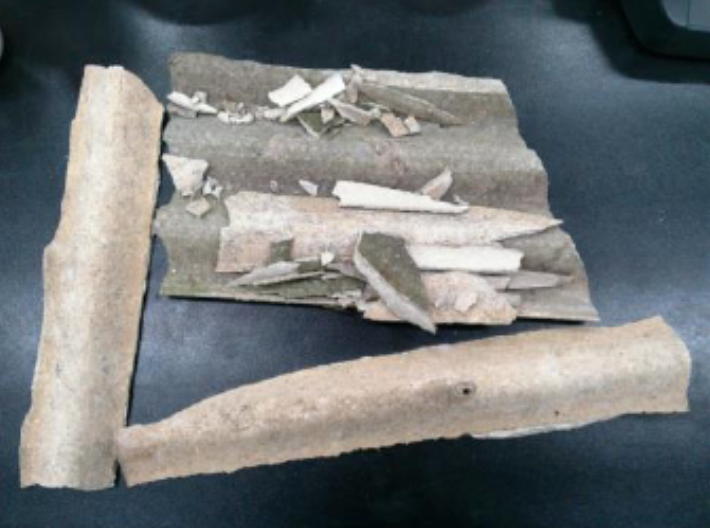
\includegraphics[width=.4\textwidth]{images/chapter2/SamplePrepOne}
}
\subfigure{
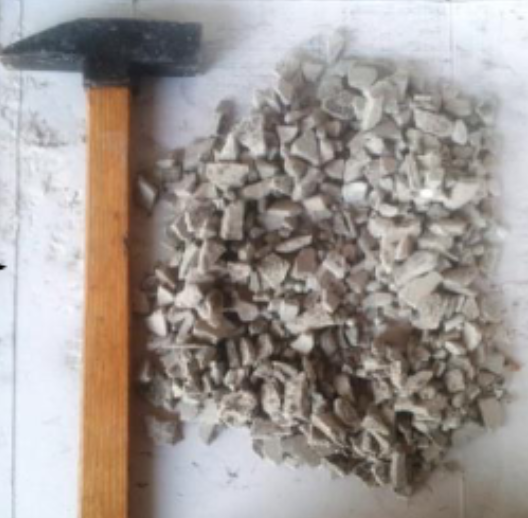
\includegraphics[width=.35\textwidth]{images/chapter2/SamplePrepTwo}
}
\subfigure{
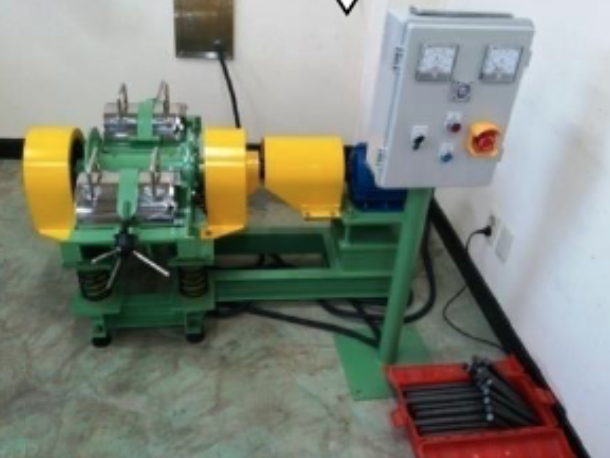
\includegraphics[width=.4\textwidth]{images/chapter2/SamplePrepThree}
}
\subfigure{
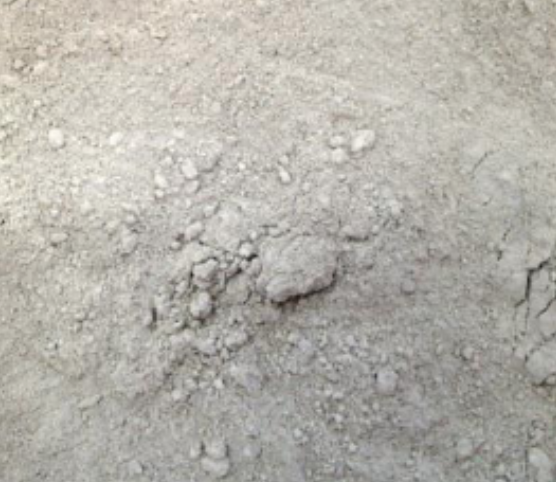
\includegraphics[width=.35\textwidth]{images/chapter2/SamplePrepFour}
}
\caption{On the upper left image the raw material is seen that needs to be screened for asbestos. In the upper right image the raw material has been processed in a first step manually. In the left lower image a crusher is seen, that takes the pieces and processes them into fine grained powder seen in the lower right image \cite{mohammed2015}. }
\label{fig:sampleprep}
\end{figure}


There are many other asbestos detection methods and counting strategies like using certain proteins from Escherichia coli that binds strongly to chrysotile, which in turn makes chrysotile easily detectable with fluorescent microscopy \cite{kuroda2008detection}. Other current methods are Polarized Light Microscopy (PLM), X-Ray Diffraction (XRD) and Fourier Transform Infrared Spectroscopy (FTIR) \cite{campopiano2018inter}. In a current and rather big inter-laboratory study, 475 laboratories in Italy were tested if they could reliably detect asbestos fibers in several bulk materials using the above mentioned three methods of PLM, XRD and FTIR. Many laboratories (ranging from 3\% to 40\% depending on the material and asbestos fiber) were classified as unsatisfactory having made to many errors in the classification. The authors concluded that asbestos detection is a complex process that uses several different approaches depending on the material and that the experience and skill of the analyst is very important. Without proper training and a scientific approach, it is very difficult to classify asbestos accurately \cite{campopiano2018inter}. \\

There are still many other detections methodologies but they all rely on manual screening which is very time-intensive labor. Searching on Google Scholar leads to only a very few papers, that applied some sort of machine learning algorithms in combination with one of the above mentioned microscopy technologies. To the best of my knowledge there has been no work done on the specific combination of SEM and CNN architectures with transfer learning. The only paper that does something similar is from 2018 and has been written by Robson et al. \cite{robson2018fiac} and is mentioned later on. \\

Cossio et al. describe an unattended scanning electron microscopy analysis with energy dispersive spectrometry (SEM-EDS) for asbestos quantification (counting of the fibers) \cite{cossio2018innovative}. Their goal was to find an automated process to increase productivity and sensitivity. After having prepared the samples and the SEM images were taken, they needed to be binarized in order to discriminate the shapes clearly from the background. They applied thresholding for that reason and transferred the image from grayscale to a black and white image only as seen in Figure \ref{fig:binarization}.

\begin{figure}[h]
\centering
\caption{Performed binarization on the grayscale image in order to discriminate the asbestos-like structures from the background noise \cite{cossio2018innovative}. }
\subfigure{
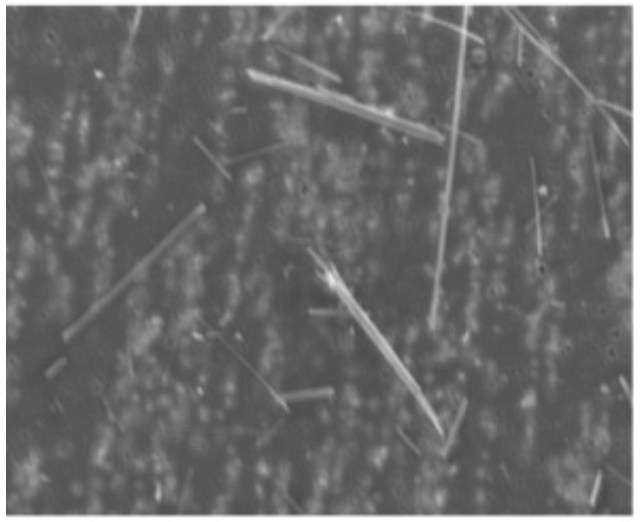
\includegraphics[width=.4\textwidth]{images/chapter2/image_original}
}
\subfigure{
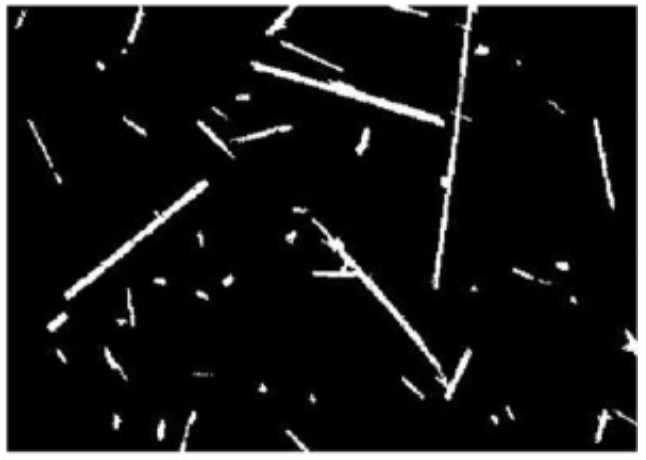
\includegraphics[width=.4\textwidth]{images/chapter2/image_binarized}
}
\label{fig:binarization}
\end{figure}

Then EDS is applied on the areas found by image binarization in order to save analytical time. Fiber morphology is then used to analytically discriminate between asbestos fibers and other minerals looking similar to asbestos. That includes length, width and aspect ratio (length/width) of the mineral structure. For the chrysotile fibers, Cossio et al. achieve 49.88\% accuracy in counting the fibers with feret diameters and 78.66\% with equivalent rectangle (ER). Both are morphology methodologies \cite{cossio2018innovative}.

Kawabata et al. use X-ray diffraction to obtain the image and dispersion staining methods to evaluate and count asbestos-like structures \cite{kawabata2009asbestos}. The dispersion staining method is a visual inspection in which white light passing through the asbestos structure is dispersed into several colors. For that reason, the fiber(s) need to be immersed into liquid. For chrysotile structures, the dispersion colors are in the range of red-purple to blue. Field interviews revealed that using this method of X-ray diffraction and dispersion staining no more than 10 samples can be examined daily. The goal of Kawabata et al. was to automate this process by examining color changes of two same images in response to dispersion staining and polarization. Relative to the aspect ratio of the fiber they achieved detection failures (false negatives) of chrysotile fibers in the examined droplets ranging from 0.35 to 0.65, meaning that 35\% to 65\% of the asbestos fibers were missed. The average percentage of incorrectly identified asbestos fibers (false positives) was approximately 20\% for chrysotile \cite{kawabata2009asbestos}. 

Moriguchi et al. used a similar approach as Kawabate et al. and used the color information from polarization (dispersion) coupled with Support Vector Machine (SVM) as the computer-based detector \cite{moriguchi2008asbestos}. To get the different properties the sample needs to be captured from two different angles. Since the two images need to be matched, the difference in angle needs to be computationally corrected for. They also found that applying SVM on every single pixel leads to many false positives and false negatives. Therefore they propose to use Conditional Random Field (CRF) on SVM outputs in order to also take the neighboring pixels into account. Miriguchi et al. reach an accuracy of 71\% with the SVM method and 78.9\% with the SVM method coupled with CRF.

Robson et al. developed a method to detect and count asbestos fibers from air samples \cite{robson2018fiac}. In contrast to soil samples, air samples are much cleaner and have less noise making the detection and counting process more easy and objective. Robson et al. used Mak R-CNN described in \cite{he2017mask} that adds a mask prediction onto the image itself showing regions that likely include the object of interest. Since Robson et al. had not enough data on hand, data augmentation and transfer learning were also applied. They were able to accurately detect 70\% of the fibers in a test set of 50 images  \cite{robson2018fiac}. \\


All in all, it is very difficult to compare the results with each other since every group uses different samples with different pre-processing methods on the image and detection or counting algorithms. It should be noted that none of the mentioned research reached an accuracy of 80\% or higher.


\section{Deeplearning Frameworks}

There are two main Deep Learning Frameworks that can readily be used. Tensorflow \cite{tensorflow} which was originally developed by researchers and engineers at Google Brain and is based on Theano. The other Deep Learning Framework is PyTorch \cite{pytorch} that was built by researchers at Facebook. They are both open source and free to use, but the flavor is quite different. While TensorFlow uses static computational graphs that need to be built prior to compilation and run in their run engine, PyTorch uses dynamic computational graphs that can be rather interpreted than compiled. Programming in PyTorch is much more pythonic whereas in TensorFlow the user needs first to get used to the way how things are handled in TensorFlow, which at times can be quite different, like building the whole computational graph in advance, using placeholders for all weights and variables, then creating a session in which the graph can be executed. Debugging in TensorFlow is more difficult since it needs at least two different debuggers to be used. One for the tensors and their values, and one for the python code itself. That makes it much less intuitive to simply debug the underlying code while keeping track of all tensors. In PyTorch, the native debugger may be used for the whole codebase, including all the variables and weights. Data parallelism is much easier to use in PyTorch since the distribution of the code and data onto all the GPU's happens automatically. Whereas in TensorFlow much more manual work and careful thought need to be applied to achieve the same behavior. Since PyTorch is one big framework it gives more the feeling of working with one framework that uses a very pythonic way to handle things. TensorFlow, on the other hand, is more like an aggregation of many libraries that work together to achieve a common goal. Although that was the case in early 2018 things are changing very fast for these frameworks. Tensorflow was much better for production environments but with PyTorch version 1.0 this advantage is closing fast \cite{pytorchOnePointZero}. Table \ref{tbl:DeepLearningFrameworks} summarizes the different qualities of both frameworks at the start of the master thesis in late summer 2018. \\

\begin{table}[t] \centering
\ra{1.3}
\caption{Different qualities of the Deep Learning Frameworks: PyTorch and TensorFlow)}
\begin{tabular}{@{}rrr@{}}
\toprule & PyTorch & TensorFlow \\
\midrule
Open-source									& + & + \\
Dynamic Computational Graph			& + & -  \\
Static Computational Graph				& - & +  \\
Easy Learning Curve							& + & -  \\
Fast developing of new Models			& + & -  \\
Production Environment					& - & + \\
Developer Community						& + & + \\
Native Visualization							& - & +  \\
Debugging										& + & -  \\
Data-Parallelisme								& + & -  \\
Framework-Feeling							& + & -  \\
Library-Aggregation							& - & +  \\

\bottomrule
\end{tabular}
\label{tbl:DeepLearningFrameworks}
\end{table}

There are some higher level frameworks like Keras \cite{keras} and DeepDIVA \cite{deepdiva} that enable many more things and faster development. Keras is built on top of TensorFlow and has many models pre-implemented. It enables the developer to very quickly start modeling a problem or apply already present architectures to new data. It does not allow the same flexibility as TensorFlow but if a new architecture needs to be designed from scratch it is done in TensorFlow than made available on Keras as to use on different datasets or different tasks. A possible counterpart for Keras is DeepDIVA that was developed at the University of Fribourg. It has been built to be used on top of PyTorch and also provides pre-implemented architectures or allows to include them in a straight-forward manner. It tackles some of the disadvantages of PyTorch versus Tensorflow like including TensorBoard Visualization to PyTorch. Development in DeepDIVA is also very pythonic and does not actually change at all since it is very tightly integrated into the PyTorch framework. Creating new architectures is or altering existing ones is straight forward.

\section{Tools}

Apart from PyTorch and DeepDIVA there is need for some other tools as well. Results and data need to be visualized and some optimization tools might be better than others.

\subsection{Visualization}

WIth CNN's it is very difficult to really know what they have learned. There are several examples that an architecture performed exceptionally well on the test set but later it was found out that it didn't really recognize the object itself but some other characteristics unrelated to the studied class. This is especially important when working with only a few classes. It is indeed very unsatisfactory from a scientific standpoint to use the accuracy alone to determine if an architecture is well suited for a problem or not. Even with other statistical parameters added, it still lacks a deeper understanding. There are several methods on how to study what a model really learns and to visualize it. Since this is still quite a young filed of research, it's quite difficult to find good libraries that can be applied to the problem. I will implement the visual toolbox by Utku Ozbulak \cite{viztoolbox} into DeepDIVA and draw conclusions from these visualizations. It remains unclear if applying this library to other architectures than AlexNet and VGG will work. From the insights gained, modifications to existing architectures might be considered. 

\subsection{SigOpt}

With all deep learning approaches it is vital to fine tune the hyper parameters like learning rate, momentum and weight-decay to the architecture and problem at hand. Often considerable amount of time is invested into this process in order to reach the best possible accuracies and reach current state-of-the-art performance. Using gridsearch for optimizing the hyper parameters would require hundreds of separate runs to find good values while only checking the value range in a very sparse manner. For the first and second baseline I did actually apply gridsearch for comparison reasons. But moving forward I applied for an academic account with SigOpt \cite{sigopt} which is a company that specializes on hyper parameter optimization. They employ Bayesian optimization which efficiently trades off exploration and exploitation of the pre-defined hyper parameters and their respective parameter space. Thus it moves quickly towards an optimal configuration that best optimizes the user's defined evaluation criterion. Common practice is to use 10 to 20 runs for each parameter which needs optimization \cite{sigoptObservationBudget}. Bayesian optimization applies mainly methods from regression models and acquisition functions, that are used together to allow fast and guided configuration search \cite{sigoptBayesian}.

\subsection{PyCharm, GIT, R and Latex}

PyCharm \cite{PyCharm} is an Integrated Development Environment for the Python programming language and has many useful features on board like code completion, static code analysis and an own debugging environment. Being able to connect through SSH with a remote server allows for modifying the remote code locally within PyCharm IDE and pushing all changes to the remote server on every save command. Remote debugging is also available with the professional license, which is free for students. Writing local scripts and integrating them with the existing PyTorch and DeepDIVA framework is easy and git is implemented directly into PyCharm which makes it easy to do almost everything within the IDE itself.
For version control, forking the original repository and adding modifications to it, GitHub \cite{GitHub} is used in combination with PyCharm and SourceTree \cite{SourceTree} as a visual GUI.
Visualizing the obtained data was done with the statistical program R \cite{statR} and RStudio \cite{rstudio} and the python libraries matplotlib and seaborn. This thesis is written in Latex.

\section{Hardware}

The hardware used is provided by the Information and Communication Department Fribourg (EIA-FR) and consists of 4 Tesla K80 Graphics Cards with each 12GB of Memory and CUDA version 10.0. It is used on an Ubuntu 18.04 machine with 32 Intel(R) Xeon(R) CPU E5-2620 cores and 126 GB of RAM.

\section{Conclusion}

For me, the most important thing was the ability to work in a very pythonic way and be able to start developing my models quickly without having to learn new frameworks. Debugging is one of the most crucial things when learning how to solve new problems and because of these two main reasons my choice fell towards PyTorch. Additionally, I decided to go with DeepDIVA on top of PyTorch. It gives me many of the advantages that applied previously only to TensorFlow like simple visualization of the results and learning process through tensorboard, but it also gives me some very useful pre-implemented architectures to start from. \\

For the visualization of the different layers of the network I decided to go with Utku Ozbulak's visualization toolbox \cite{viztoolbox}. It is implemented in PyTorch and can be applied with some code adaptations to the AlexNet and VGG models. It has many different visualization modes to chose from and is quite extensive. It also provides a heat map visualization that shows which areas of the image contributed to classifying the image one way, or the other way.\\

Gridsearch and SigOpt were both used for hyper parameter optimization initially but for the more complex architectures only SigOpt was used since it allows for more fine-grained values and leads to better results within a smaller time frame. \\